\documentclass{VUMIFPSkursinis}
\usepackage{algorithmicx}
\usepackage{algorithm}
\usepackage{algpseudocode}
\usepackage{amsfonts}
\usepackage{amsmath}
\usepackage{bm}
\usepackage{caption}
\usepackage{color}
\usepackage{float}
\usepackage{graphicx}
\usepackage{listings}
\usepackage{subfig}
\usepackage{wrapfig}
\usepackage[backend=biber]{biblatex}

% Titulinio aprašas
\university{Vilniaus universitetas}
\faculty{Matematikos ir informatikos fakultetas}
\department{Programų sistemų katedra}
\papertype{Kursinis darbas}
\title{Didelių duomenų srautų analizė, anomalijų aptikimas}
\titleineng{Large data flow analysis, detection of anomalies}
\status{3 kurso 3 grupės studentas}
\author{Jokūbas Rusakevičius}
% \secondauthor{Vardonis Pavardonis}   % Pridėti antrą autorių
\supervisor{dr. Vytautas Valaitis}
\date{Vilnius – \the\year}

% Nustatymai
\setmainfont{Palemonas}   % Pakeisti teksto šriftą į Palemonas (turi būti įdiegtas sistemoje)
\bibliography{bibliografija}
%\addbibresource{bibliografija.bib}

\begin{document}
\maketitle

\tableofcontents

\sectionnonum{Įvadas}
Surenkamų duomenų kiekiai nuolatos didėja ir gerokai lenkia žmonių sugebėjimą juos apdoroti, peržiūrėti ar analizuoti. Didžiosios socialinių tinklų kompanijos Twitter, Facebook ir LinkedIn praneša kiekviena atskirai fiksuojanti iki 12 milijonų įvykių per sekundę \cite{twitter, facebook, linkedin}. Taip pat, vis daug duomenų yra surenkama iš automatizuotų duomenų šaltinių (pvz.: „Dalykų Interneto“ (angl. „Internet of Things“)). Kylantis automatizuotų duomenų šaltinių populiarumas, pinganti techninė įranga, išvystyti komunikaciniai tinklai bei mažėjančios duomenų saugojimo kainos paskatino dešimčių milijardų dolerių komercines investicijas šių technologijų vystimui \cite{iof_investments}. Numatoma, kad kiekvienais metais bendras duomenų kiekis augs po 40\% \cite{iof}.



%Įvade apibūdinamas darbo tikslas, temos aktualumas ir siekiami rezultatai.
%Darbo įvadas neturi būti dėstymo santrauka. Įvado apimtis 1–2 puslapiai.

% \section{Medžiagos darbo tema dėstymo skyriai}
% Medžiagos darbo tema dėstymo skyriuose pateikiamos nagrinėjamos temos detalės:
% pradinė medžiaga, jos analizės ir apdorojimo metodai, sprendimų įgyvendinimas,
% gautų rezultatų apibendrinimas. Šios dalies turinys labai priklauso nuo darbo
% temos. Skyriai gali turėti poskyrius ir smulkesnes sudėtines dalis, kaip
% punktus ir papunkčius.

% Medžiaga turi būti dėstoma aiškiai, pateikiant argumentus. Tekstas dėstomas
% trečiuoju asmeniu, t.y. rašoma ne „aš manau“, bet „autorius mano“, „autoriaus
% nuomone“. Reikėtų vengti informacijos nesuteikiančių frazių, pvz., „...kaip jau
% buvo minėta...“, „...kaip visiems žinoma...“ ir pan., vengti grožinės literatūros
% ar publicistinio stiliaus, gausių metaforų ar panašių meninės išraiškos
% priemonių.

% \subsection{Poskyris}
% Citavimo pavyzdžiai: cituojamas vienas šaltinis \cite{PvzStraipsnLt}; cituojami
% keli šaltiniai \cite{PvzStraipsnEn, PvzKonfLt, PvzKonfEn, PvzKnygLt, PvzKnygEn,
% PvzElPubLt, PvzElPubEn, PvzMagistrLt, PvzPhdEn}.

\section{MacroBase duomenų analizės sistema}
MacroBase yra didelių ir/ar greitų duomenų ar duomenų srautų analitinė stebėjimo sistema. 

\sectionnonum{Rezultatai ir išvados}
Rezultatų ir išvadų dalyje turi būti aiškiai išdėstomi pagrindiniai darbo
rezultatai (kažkas išanalizuota, kažkas sukurta, kažkas įdiegta) ir pateikiamos
išvados (daromi nagrinėtų problemų sprendimo metodų palyginimai, teikiamos
rekomendacijos, akcentuojamos naujovės).

\printbibliography[heading=bibintoc]
% Šaltinių sąraše nurodoma panaudota
% literatūra, kitokie šaltiniai. Abėcėlės tvarka išdėstomi darbe panaudotų
% (cituotų, perfrazuotų ar bent paminėtų) mokslo leidinių, kitokių publikacijų
% bibliografiniai aprašai.  Šaltinių sąrašas spausdinamas iš naujo puslapio.
% Aprašai pateikiami netransliteruoti. Šaltinių sąraše negali būti tokių
% šaltinių, kurie nebuvo paminėti tekste.

% \sectionnonum{Sąvokų apibrėžimai}
\sectionnonum{Santrumpos}
Sąvokų apibrėžimai ir santrumpų sąrašas sudaromas tada, kai darbo tekste
vartojami specialūs paaiškinimo reikalaujantys terminai ir rečiau sutinkamos
santrumpos.

\appendix  % Priedai
% Prieduose gali būti pateikiama pagalbinė, ypač darbo autoriaus savarankiškai
% parengta, medžiaga. Savarankiški priedai gali būti pateikiami ir
% kompaktiniame diske. Priedai taip pat numeruojami ir vadinami. Darbo tekstas
% su priedais susiejamas nuorodomis.

%\section{Niauroninio tinklo struktūra}
%\begin{figure}[H]
%    \centering
%    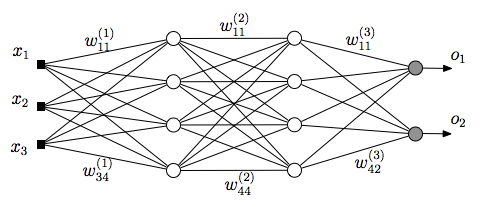
\includegraphics[scale=0.5]{img/MLP}
%    \caption{Paveikslėlio pavyzdys}
%    \label{img:mlp}
%\end{figure}
%
%
%\section{Eksperimentinio palyginimo rezultatai}
%% tablesgenerator.com - converts calculators (e.g. excel) tables to LaTeX
%\begin{table}[H]\footnotesize
%  \centering
%  \caption{Lentelės pavyzdys}
%  {\begin{tabular}{|l|c|c|} \hline
%    Algoritmas & $\bar{x}$ & $\sigma^{2}$ \\
%    \hline
%    Algoritmas A  & 1.6335    & 0.5584       \\
%    Algoritmas B  & 1.7395    & 0.5647       \\
%    \hline
%  \end{tabular}}
%  \label{tab:table example}
%\end{table}

\end{document}
